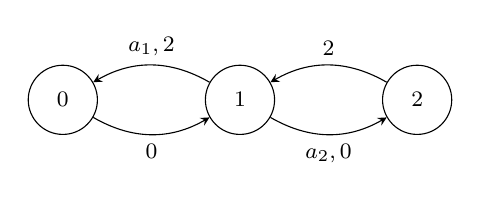
\begin{tikzpicture}[thin, scale=0.75]
  % Nodes
  \draw (-3,0) node(0) [circle,draw,minimum size=25] {\footnotesize \(0\)};
  \draw (0,0)  node(1) [circle,draw,minimum size=25] {\footnotesize \(1\)};
  \draw (3,0)  node(2) [circle,draw,minimum size=25] {\footnotesize \(2\)};

  % Edges
  \path[thin, ->, bend right, >=stealth] (1) edge[above] node {\footnotesize\(a_{1},2\)} (0);
  \path[thin, ->, bend right, >=stealth] (2) edge[above] node {\footnotesize\(2\)} (1);
  \path[thin, ->, bend right, >=stealth] (0) edge[below] node {\footnotesize\(\alert{0}\)} (1);
  \path[thin, ->, bend right, >=stealth] (1) edge[below] node {\footnotesize \(a_{2},\alert{0}\)} (2);

  % \draw (-1.5,0) node[] { A };
  % \draw (1.5,0) node[] { B };
\end{tikzpicture}

%%% Local Variables:
%%% mode: latex
%%% TeX-master: "../presentation"
%%% End:


